\taskpic{ Узкая трубка постоянного сечения образует квадрат со
  стороной $l$, закреплённый в вертикальной плоскости. Трубка
  заполнена равными объёмами двух не проникающих друг в друга
  жидкостей с плотностями $\rho_1$ и $\rho_2<\rho_1$. Вначале более
  плотная жидкость заполняла верхнюю часть трубки. В некоторый момент
  жидкости пришли в движение. Найти их максимальную скорость. Трением
  пренебречь. }
{
  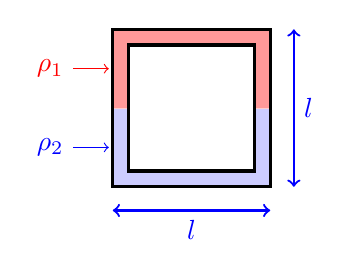
\begin{tikzpicture}
    \draw[blue!20,fill=blue!20] (1,0) -- (3,0) -- (3,1) -- (2.8,1) --
    (2.8,0.2) -- (1.2,0.2) -- (1.2,1) -- (1,1) -- cycle;
    \draw[red!20,fill=red!40] (1,1) -- (1,2) -- (3,2) -- (3,1) --
    (2.8,1) -- (2.8,1.8) -- (1.2,1.8) -- (1.2,1) -- cycle;
    \draw[very thick] (1,0) -- (3,0) -- (3,2) -- (1,2) -- cycle;
    \draw[very thick] (1.2,0.2) -- (2.8,0.2) -- (2.8,1.8) -- (1.2,1.8)
    -- cycle;
    \draw[thick,blue,<->] (1,-0.3) -- (3,-0.3) node[below,midway,blue]
    {$l$};
    \draw[thick,blue,<->] (3.3,0) -- (3.3,2) node[right,midway,blue]
    {$l$};
    \draw[blue,->] (0.5,0.5) node[left,blue] {$\rho_2$} -- (0.95,0.5);
    \draw[red,->] (0.5,1.5) node[left,red] {$\rho_1$} -- (0.95,1.5);
  \end{tikzpicture}
}
% Новосиб, 1.72
